\documentclass[12pt]{article}
\usepackage[a4paper, total={6in, 8in}]{geometry}
\usepackage{setspace}
\usepackage{amsmath}
\usepackage{amssymb}
\usepackage{witharrows}
\usepackage{lipsum}
\usepackage{indentfirst}
\usepackage{mathtools}
\usepackage{layout}
\usepackage{xcolor}
\usepackage{amsmath}
\usepackage{systeme}
\usepackage{blindtext}
\usepackage{sidenotes}
\usepackage{multicol}
\usepackage{fancyhdr}
\usepackage{indentfirst}
\usepackage{systeme}
\usepackage{hyperref}
\usepackage{natbib}
\usepackage{indentfirst}
\usepackage{mwe}
\usepackage{epigraph}
\usepackage[skip=10pt plus1pt]{parskip}
\WithArrowsOptions{displaystyle,tikz=blue}

\doublespacing
\begin{document}
\pagenumbering{gobble}
\begin{titlepage}
	\centering
	\vspace{1cm}
	{\Large \textsc{``Mathematics: Analysis And Approaches" Extended Essay}\par}
	\vspace{1.5cm}
	{\huge\bfseries The Game Of Cat \& Swan, Applications Of Complex Numbers\par}
	\vspace{2cm}
	\vfill
	\vfill
	{\large \today, 1818 words\par}
\end{titlepage}

\clearpage
\pagenumbering{arabic}
\tableofcontents
\newpage

%%% NOTES TO SELF:
%%% maybe explain what opposite means on a circle
%%% assume the Cat doesn't move if the Swan is directly in the centre

\section{Introduction}
\subsection{Abstract}
The research question of this Mathematics Extended Essay is the following problem:

\emph{Imagine a Swan in a middle of a perfectly circular unit lake. Standing on the edge is a hungry Cat. The Cat is after the Swan and the Swan's goal is to escape. The best route is flight, and yet it can only take off from land. The Cat on land is 4 times faster than the Swan on water. Can the Swan escape the Cat and if yes, what trajectory does it need to follow?}

In investigating this question I first ensured that it has a solution using simple direct proofs, then expressed the variables in terms of complex numbers to ease visualising it and used my knowledge I've collected during the DP years. At any point reading this you may refer to the table of all variables in the Appendix.

\section{Solution}
There are several versions of the problem with different species chasing eachother around, but alas I could not trace down the source. Versions of this problem can be found under the names of "A Lady And A Monster"\cite{ladyandmonster}, "Game Of Cat And Mouse"\cite{Catandmouse} and others. The general premise and numerical values stay the same across interpretations. 

My primary reason for choosing to focus on this specific problem came from my strong desire to find an analytical solution to it. Eversince I saw it in a YouTube video\cite{Catandmouse}, I was excited to have it on my radar, the Extended Essay offered me a window of opportunity. I also enjoy spending my free time pondering problems like that, although they are usually of computer science ilk. This problem turned out to be especially difficult, even though most of the steps and theorems can be outlined on a paper towel, all require deep insights into how the problem works.

We will assume both animals to be acting \textit{nearly optimally}, so are choosing whichever option gives them the best result in the moment, or when two or more solutions are equally optimal we will make sure to define one of them to always pick. In Cat's case it is trying to be closer to the Swan, since its "win condition" is essentially having the same position as the Swan on the lake border. I will conjecture that the Cat will always pick the shortest path to any point $p$, in hopes that this decision is obvious.

\textbf{Theorem}: The best way for the Cat to act is to move closer to the Swan.

\textbf{Proof}: Assume the Swan has velocity $V$ and if it was to keep that velocity unchanged it would reach the lake shore at point $p$. Assume the cat is moving towards some other point $p'$, such that $p' \neq p$. If $p$ does not belong to an arc $C$ on the lake spanning from the Cat's current position to point $p'$, then the Swan is guaranteed to win. In case that $p \in C$, the Swan can direct it velocity at $-V$, which will correspond to a point $-p$ that is not on the arc $C$. $\blacksquare$

The same logic, sadly, does not express the variety of the Swan's potential strategies, since it's goal is not to actually get away from the Cat, but to reach the shore without being caught. One of the first things you can do when approaching such question is look at whether it even is solvable.

\begin{center}
	\begin{tikzpicture}[scale=2]
		\draw (0,0) circle [radius=1];
	\end{tikzpicture}
\end{center}

\subsection{The Dash Distance}

The simplest strategy for the Swan is to swim towards the shore in a straight line without ever changing direction, it is the shortest path after all. We will denote the velocities of the Swan and the Cat as $V$ and $V'$ respectively. The time $t$ it takes the Swan to reach the shore will be $\frac{r}{V}$. In Cat's case it entirely depends on the point, for example to reach the point opposite to it's current is going to take $t' = \frac{\pi r}{V'} = \frac{\pi r}{4V}$. Notice that even if the Swan swims directly away from the Cat's initial position it will be caught:

\textbf{Theorem:} The Cat will outrun the Swan if the Swan swims directly opposite to the Cat's initial position.

\textbf{Proof:} Assume 
\begin{center}
$\begin{WithArrows}
\text{t} &< \text{t'} \Arrow{Substitute}\\
\frac{\pi r}{V'} &< \frac{r}{V} \Arrow{$V' = 4V$}\\
\frac{\pi r}{4V} &< \frac{r}{V} \Arrow{$\square \cdot \frac{V}{r}$}\\
\frac{\pi}{4} &< 1 \hspace{10pt} \blacksquare
\end{WithArrows}$
\end{center}

We see that the just dashing to the edge won't work for the Swan if it's in the middle, but we can imagine alternative conditions. If the Swan is closer to the edge, surely it could be faster than the Cat?

Assume the Swan is such distance $d$ away from edge and directly opposite the Cat, so that it can safely reach the edge. That would mean that the time it takes the Swan to reach the edge is shorter, than the time it takes the Cat to reach the same point. It of course depends on the position of the Cat, but let it be exactly opposite the Swan. It can be expressed as $\frac{d}{V} < \frac{\pi r}{4V} \Leftrightarrow  d < \frac{\pi}{4}r$.

\subsection{The Freedom Circle}

Now the question is whether it is even possible to get to that point. We can turn our attention to the angular velocities of the animals, since both of them are moving around the circle. If the distance of the Swan from the center is $D = r - d$, the Swan has the angular velocity of $\omega = \frac{V}{D}$ and the Cat has angular velocity $\omega' = \frac{4V}{r}$. Notice how the velocity of the Cat is essentially constant, but the velocity of the Swan is controlled by its distance from the center $D$. Based on this we can solve for $D$, at which the Swan is angularly faster than the Cat.

\begin{center}
$\begin{WithArrows}[jot=2ex]
\frac{V}{D} &> \frac{4V}{r} \Arrow{$\square^{-1}$}\\
\frac{D}{V} &< \frac{r}{4V} \Arrow{$\square \cdot {V}$}\\
D &< \frac{r}{4} \Arrow{$D = r - d$}\\
r - d &< \frac{r}{4} \Arrow{$\square - r$}\\
- d &< \frac{r}{4} - r  \Arrow{$\square \cdot (-1)$}\\
d &> r - \frac{r}{4}
\end{WithArrows}$
\end{center}

So far all points that are $D$ or less away from the center (inside the "freedom" circle of radius $D$)the Swan is faster, so I claim it can occupy any position inside, positioning itself anywhere relative to the Cat.

Notice that there can exist such $d$ that $r - \frac{r}{4} < d < \frac{\pi}{4}r$. Given that $r = 1$ we get to know that the distance of the Swan from the edge has to be $\frac{3}{4} < d < \frac{3.14\dots}{4}$. The set of all positions for the Swan to be in forms an "safety" annulus inside the circle. When the Swan is inside this annulus and the Cat is opposite the Swan, it may dash to the edge of the lake and flee, so the trajectory must exist.

There exists an infinite amount of viable trajectories, since for every possible trajectory, the Swan can make a lap inside the "freedom" circle one more time, giving us a new trajectory. 

\subsection{Describing Velocity}

Next we may look at getting to the edge of the "safety" annulus. For a successful escape the Swan has to exit it at such point, that it's directly opposite the Cat. Over an infinitesimal amount of time $\Delta t$ the Swan can travel a total distance of $s = V \Delta t$. Assume the Swan is somewhere inside the "freedom" circle, then the Cat moves at $\omega' = \pm \frac{4V}{r}$. The Cat can move either clockwise or counterclockwise, since at all times there are two paths to its desired point and the Cat is always going to choose the shortest (except for the case when cat is directly opposite, since then two paths have equal lengths, when that happens we will assume the cat to move counterclockwise $\omega' > 0$).

In this case in order to compensate for the Cat's movement (remain opposite to it) the Swan has to move the same angle in \textit{the same direction around the clock, but opposite in terms of coordinates}. Since the magnitude of the velocity vector should remain $V$, we can express it as two vectors: moving away from the center to exit the "freedom" circle ($V_\alpha$) and compensation for Cat's movement ($V_{\omega'}$). If compensation is $V_{\omega'} = \omega' \cdot D$, we can solve for the away velocity ($V_\alpha$) as follows:

\begin{center}
$\begin{WithArrows}[jot=2ex]
V &= \sqrt{(\omega'D)^2  + V_\alpha^2} \Arrow{$\square^2$}\\
V^2 &= (\omega'D)^2  + V_\alpha^2 \Arrow{$\square - (\omega'D)^2$}\\
V_\alpha^2 &= V^2 - (\omega'D)^2 \Arrow{$\sqrt{\square}$}\\
V_\alpha &= \sqrt{V^2 - (\omega'D)^ 2}
\end{WithArrows}$
\end{center}

\begin{center}
	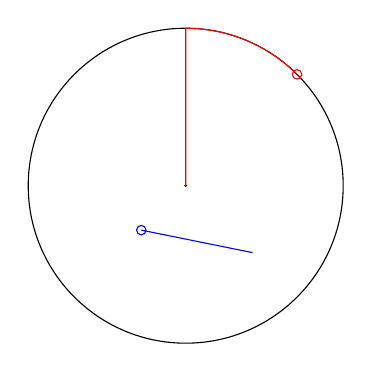
\begin{tikzpicture}[scale=2]
		\draw (0,0) circle [radius=1];
		\fill[color=black] (0,0) circle [radius=0.01];
		\draw[color=red] (0.707,0.707) circle [radius=0.03];
		\draw[color=blue] (-0.282,-0.282) circle [radius=0.03];
		\draw[color=red] (0.707,0.707) 
		arc[start angle = 45, end angle = 90, radius=1]
		(0, 0) -- (0, 1);
		\draw[color=blue] (-0.282, -0.282) -- (0.425, -0.425);
		
	\end{tikzpicture}
\end{center}

\subsection{Describing Position}

When describing the motion of objects in a 2D plane like in our case it only makes sense to use vectors, however, since we often deal with angles an rotations a polar complex coordinate system is a lot more appropriate. We will define $i$ such that $i = \sqrtsign{-1}$ and assume 1 and $i$ to be the vector bases for $\{z \in \mathbb{C}: z = 1x + iy\}$. The \textit{set} $\mathbb{C}$ is isomorphic to $\mathbb{R}^2$, so the two are interchangable in this context. %TODO: proof?% 

We can introduce a polar coordinate system to get the velocities for the Swan or the Cat as complex numbers $\vec{V}$ and $\vec{V}'$ respectively. Since the Cat always moves tangentially, let $\theta$, the angle between the Cat's position and the x-axis, then its velocity will always be directed at angle $\theta \pm \pi$ relative to the x-axis (tangentially to the circle, counterclockwise or clockwise depending on the $\pm \pi$).

To get the angle we can imagine the complex number to be describing a line, since the real part is usually considered the x coordinate and the imaginary is the y, the slope of the line going through that point is $\frac{y}{x}$, so for $1x + iy$ it is $\tan \theta = \frac{y}{x}$, so to get the angle we apply $\arctan$ to both sides, that yields $\theta = \arctan{\frac{y}{x}}$, the definition of the \textit{argument} or the \textit{phase} of a complex number denoted $\arg z$. There is an issue with purely imaginary numbers (when $\Re (z) = 0$), since in that case $\arg$ would be undefined. To avoid this issue we may extend this function to the following: $$
\arg (z) = \left\{ 
		\begin{aligned}
			\pi						,\hspace{4pt}&  z = 0 + |z|i\\
			-\pi					,\hspace{4pt}&  z = 0 - |z|i\\
			\arctan {\frac{\Im (z)}{\Re (z)}}	,\hspace{4pt}&	\text{otherwise}\\
		\end{aligned}
	\right.$$

To decide whether to move clockwise or counterclockwise the Cat can use the cross product of its own and the Swan's positions $P \times P'$, specifically the imaginary component. Due to the properties of the cross product it will always yield a vector perpendicular to the initial two, but since we are restricted to be inside a complex plane, the only vector component is imaginary. Given that complex numbers are vectors with bases $1$ and $i$, the cross product is just the determinant of a joined matrix of vectors: $P \times P' = (a + ib) \times (c + id) = \det \bigl[ \begin{smallmatrix} 
	a & c\\
	ib & id 
  \end{smallmatrix} \bigr] = iad - ibc = i(ad - bc)$.

From that we see that the only vector component is, indeed, imaginary, so we define $p_\times = \Im{(P \times P')}$ and verify that it's sign will match the optimal direction:

\begin{tabular*}{\linewidth}{|l|c|r|}
	
\end{tabular*}

One of the problems that may also arise is that the cross product of two collinear\cite{vectorterminology} vectors is $0$, in our case that would happen when the Swan is either moving directly at the Cat or directly away. However, since we defined the Swan's strategy to require always moving in the opposite direction, we can omit the case of the vectors being collinear and parallel\cite{vectorterminology} and only focues the collinear and antiparallel\cite{vectorterminology} case.

Since scaling the cross product would also influence the magnitude of the velocity vector we will use the signum function. $$\text{sgn}(x) = \left\{ 
	\begin{aligned}
		-1&, x < 0\\
		0&, x = 0\\
		1&, x > 0
	\end{aligned}
\right.$$

The main issue with this classic definition is that it is $0$ at $x = 0$, in our problem domain this would correspond to the Cat getting stuck when it is opposite the Swan, for that purpose we will define another function, to insist going counterclockwise in an ambigous case:$$\text{sgn}_+(x) = \left\{ 
	\begin{aligned}
		-1&, x < 0\\
		1&, x \geq 0
	\end{aligned}
\right.$$

Given all of the above, the final velocity vector of the Cat is the following: $$
\vec{V}' = 4 \cdot \text{ sgn}_+ (p_\times) \cdot (\cos(\theta) + i \sin(\theta))
$$

We had to use a clever $\text{sgn}$ function to describe the direction, however, I CONJECTURE THAT THE SWAN ONLY MOVES IN ONE DIRECTION AND THAT DIRECTION IS COUNTERCLOCKWISE, END OF STORY. There is no reason for the Cat to change direction ever.

The Swan on the other hand will have to decide on the strategy depending on the distance $D$ from the center. When dashing away all of it's velocity will be directed away from the center, exactly where the magnitude of it's position $P$ is directed.

\begin{equation*}
	\vec{V} = \left\{ 
		\begin{aligned}
			\frac{\vec{V}'}{4} \cdot (i V_\alpha  - \omega' D) \\
			\frac{P}{|P|}, 
		\end{aligned}
	\right.
\end{equation*}

\subsection{Lake Shapes \& Polar Curves}

Since the case of a circular lake is solved we may generalize the problem to a broader case, specifically the case of any lake shape.

\section{Conclusion}
Glad I did it with \LaTeXe\cite{latex2e}, will continue using it.

\section*{Appendix}

\begin{tabular}{|l|l|}
\hline
\textbf{Variable} & \textbf{Purpose}\\
\hline
$r \in {\mathbb{R}^+}$ & The radius of the lake\\
$d \in \{x \in \mathbb{R^+}: 0 \leq x < r \}$ & Distance of the Swan from the edge\\
$D = r - d$ & Distance of the Swan from the center, magnitude of position\\
$V \in {\mathbb{R}^+}$ & Magnitude of the Swan's velocity\\
$V' = 4V$ & Magnitude of the Cat's velocity\\
$\vec{V}' \in \mathbb{C}$ & Complex velocity vector of the Cat\\
$\vec{V} \in \mathbb{C}$ & Complex velocity vector of the Swan\\
$\omega \in \mathbb{R}_{2\pi}$ & The angular velocity of the Swan\\
$\omega' \in \mathbb{R}_{2\pi}$ & The angular velocity of the Cat\\
$V_{\omega'} \in \mathbb{R^+}$ & Swan's linear compensation for Cat's angular velocity\\
$V_\alpha \in \mathbb{R^+}$ & Swan's velocity component directed away from the Cat\\
$P \in \mathbb{C}$ & Position of the Swan\\
$P' \in \mathbb{C}$ & Position of the Cat\\
$\theta$ & Angular distance of the Cat from the x-axis\\
$p_\times$ & Cross product of the Cat's and Swan's positions\\
\hline
\end{tabular}
\vspace{12pt}

\bibliographystyle{plain}
\bibliography{sources}
\end{document}
